\documentclass{beamer}
%\usetheme{CambridgeUS}
\usetheme{Warsaw}
\usepackage[utf8]{inputenc}
\usepackage{polski}
\usepackage[polish]{babel}
\usepackage[OT4]{fontenc}
\usepackage{graphicx}
\usepackage{listings}

\newtheorem{hypothesis}{Hipoteza}

\author{Konrad Gądek}
\institute[AGH]{Akademia Górniczo-Hutnicza}
\date{30.~listopada 2010}
\title{Common Lisp w obecnym świecie}
\begin{document}

% Ważne:	* wyraźnie zaznaczyć postawioną hipotezę/temat prezentacji
%			  i~starać się ją udowadniać
%			* zaznaczyć ``so what-y'' we wstępie i~w~podsumowaniu
% 1. Wstęp
%	O~czym będzie mowa a~o~czym nie
%		``Na dzisiejszej prezentacji dowiecie się Państwo...''
%	Hipoteza W-S
%		Język ang vs Polski
%		Teoria kodów Bernsteina
%		Stacje benzynowe w~ameryce
%		Języki egzotyczne? (japoński, chiński)
%	Co to jest język?
%	Jak to się ma do komputerów?
%	Podsumowanie
% 2. Common Lisp
%	Notacje w~matematyce
%		Notacja infiksowa
%			Zapis operatorów wieloargumentowych
%		Od notacji infiksowej do prefiksowej...
%		...aż do języka Common Lisp
%	Co jeszcze warto wiedzieć o~języku?
%		Pętle, funkcje, instrukcje warunkowe
%	Kilka prostych przykładów
%	Co wyróżnia CL? Paradygmaty
% 3. Makra
%	Dlaczego tyle nawiasów?
%	Jakie są możliwości? -- tzw. ``drabina'' abstrakcji (por. z~C/C++)
%	Bardzo prosty przykład
%	Bardzo fajny przykład
%	Co dalej? Co to jest DSL?
% 4. Przykłady programów
%	Pomoce naukowe czyli programy pomocnicze do nauki matematyki dyskretnej
%	Problemy komiwojażera -- rysowanie sieci MLM
%		Sposób długi (C-like)
%		Sposób krótszy
%	(LOL) Jednostki w~programie
%	Papcio Knuth prezentuje: DXL
%	Pokonując mrówki
% 5. Porównanie wydajności
%	Kompromis pomiędzy szybkością pisania a~szybkością programu
%	C++ -- wydajne od początku, CL -- wydajne kiedy chcemy
%	Wydajny kod C++ vs. wydajny kod CL -- przytoczenie wyników prac
% 6. Podsumowanie
%	Dla kogo CL? W~jakich przypadkach?
%		Graham: historyjka o~sklepie internetowym
%		reddit -- wcale nie FAIL języka
%		wykorzystanie języka przy pisaniu AI
%	A~jeśli nie będziemy korzystać z~CL?
%	Further reading

\begin{frame}[plain]
	\titlepage
\end{frame}

\section*{Wstęp}
\begin{frame}{Plan prezentacji}
	Na dzisiejszej prezentacji nie będzie\ldots:
	\begin{enumerate}
		\item{\ldots kompletnego kursu języka Common Lisp}
		\item{\ldots opisu wszystkiego co powoduje, że Common Lisp jest
			taki potężny (CLOS, makra, restarts/continuations, DLS,\ldots)}
	\end{enumerate}
	\emph{Postaram się} za to opowiedzieć:
	\begin{enumerate}
		\item{dlaczego warto się nauczyć języka Common Lisp}
		\pause \item{dlaczego Lisp przetrwał ponad 52 lata}
		\pause \item{dlaczego indianie nie powinni pracować na
					stacji benzynowej, jak zwracać się do
					własnych dzieci i~dlaczego warto zostać
					inspektorem ubezpieczeniowym}
	\end{enumerate}
\end{frame}


\section{Trochę teorii}

\begin{frame}{Języki}
	\begin{block}{Język}
		Ukształtowany społecznie system budowania wypowiedzi, używany w~procesie komunikacji
		interpersonalnej.
	\end{block}
\end{frame}

\begin{frame}{Hipoteza Sapira\dywiz Whorfa}
 	\begin{alertblock}{Prawo relatywizmu językowego}
		W~skrócie: używany język wpływa w~mniejszym lub większym
		stopniu na sposób myślenia.
	\end{alertblock}
	\pause
	\begin{block}{Przykład 1. - o~niewiernym mężu}
		W~polsce: idę do sąsiada/sąsiadki\\
		W~anglii: I'm going to my neighbour (bez określenia płci)
	\end{block}
	\pause
	\begin{block}{Przykład 2. - jaki jest Twój nr~telefonu?}
		n\v i de di\`an hu\`a h\`ao m\v a sh\v i du\=o sha\v o --- Ty-od-elektryczny-rozmowa-numer-porządkowy-jest-jaki-duży?
	\end{block}
\end{frame}

\begin{frame}{Grzebienie a~inspektor ubezpieczeniowy}
	Grzebień drewniany z~rączką:
	\begin{figure}
	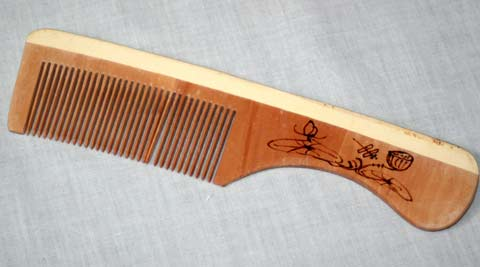
\includegraphics[scale=0.1]{grzebien_drewniany_raczka}
	\end{figure}
	Grzebień plastikowy z~rączką:
	\begin{figure}
	
\includegraphics[scale=0.1]{grzebien_plastik_raczka}
	\end{figure}
	Grzebień plastikowy:
	\begin{figure}
	
\includegraphics[scale=0.1]{grzebien_plastik}
	\end{figure}
\end{frame}

\begin{frame}{Bernstein i~angielskie dzieci}
	\begin{alertblock}{Teoria kodów Bernsteina}
		W~różnych od siebie klasach funkcjonują odmienne typy schematów językowych (kodów).
	\end{alertblock}
	Wyniki potwierdzone w~latach 70. w~Polsce.
\end{frame}

\begin{frame}{Języki}
	\begin{block}{Język}
		Ukształtowany społecznie system budowania wypowiedzi, używany w~procesie komunikacji
		interpersonalnej.
	\end{block}
	\begin{block}{Język programowania}
		Zbiór zasad określających, kiedy ciąg symboli tworzy program oraz jakie
		obliczenia opisuje.
	\end{block}
	\pause
	\alert{Języki (programowania) są narzędziem!}
\end{frame}

\begin{frame}{Paul Graham i~Blub oraz rekurencja w~Basicu}
	Jeżeli\ldots
	\begin{enumerate}
		\item{jeden język może być lepszy od drugiego\ldots}
		\pause \item{potrafimy jedynie stwierdzić, że język X jest gorszy od języka Blub\ldots}
		\pause \item{nie potrafimy stwierdzić, że język Y jest lepszy od Bluba -- możemy
			tylko stwierdzić, że \emph{jest jakiś dziwny}}
	\end{enumerate}
	\pause
	To:
	\begin{enumerate}
		\item{jedynie ucząc się Y potrafimy stwierdzić, czy Y~$>$~Blub}
		\pause \item{jedynie ucząc się Y stwierdzimy, czy jego funkcja $\alpha$
			jest faktycznie przydatna}
	\end{enumerate}
	\pause
	\ \\
	``That language [Basic] didn't even support recursion. It's hard to imagine writing
	programs without using recursion, but I~didn't miss it at the time. I~thought in
	Basic.''
\end{frame}

\begin{frame}{Wniosek}
	\begin{alertblock}{Oczywiste?}
		Są lepsze i~gorsze języki programowania!
	\end{alertblock}
\end{frame}

\begin{frame}{Jak to widzą programiści?}
	\begin{figure}
		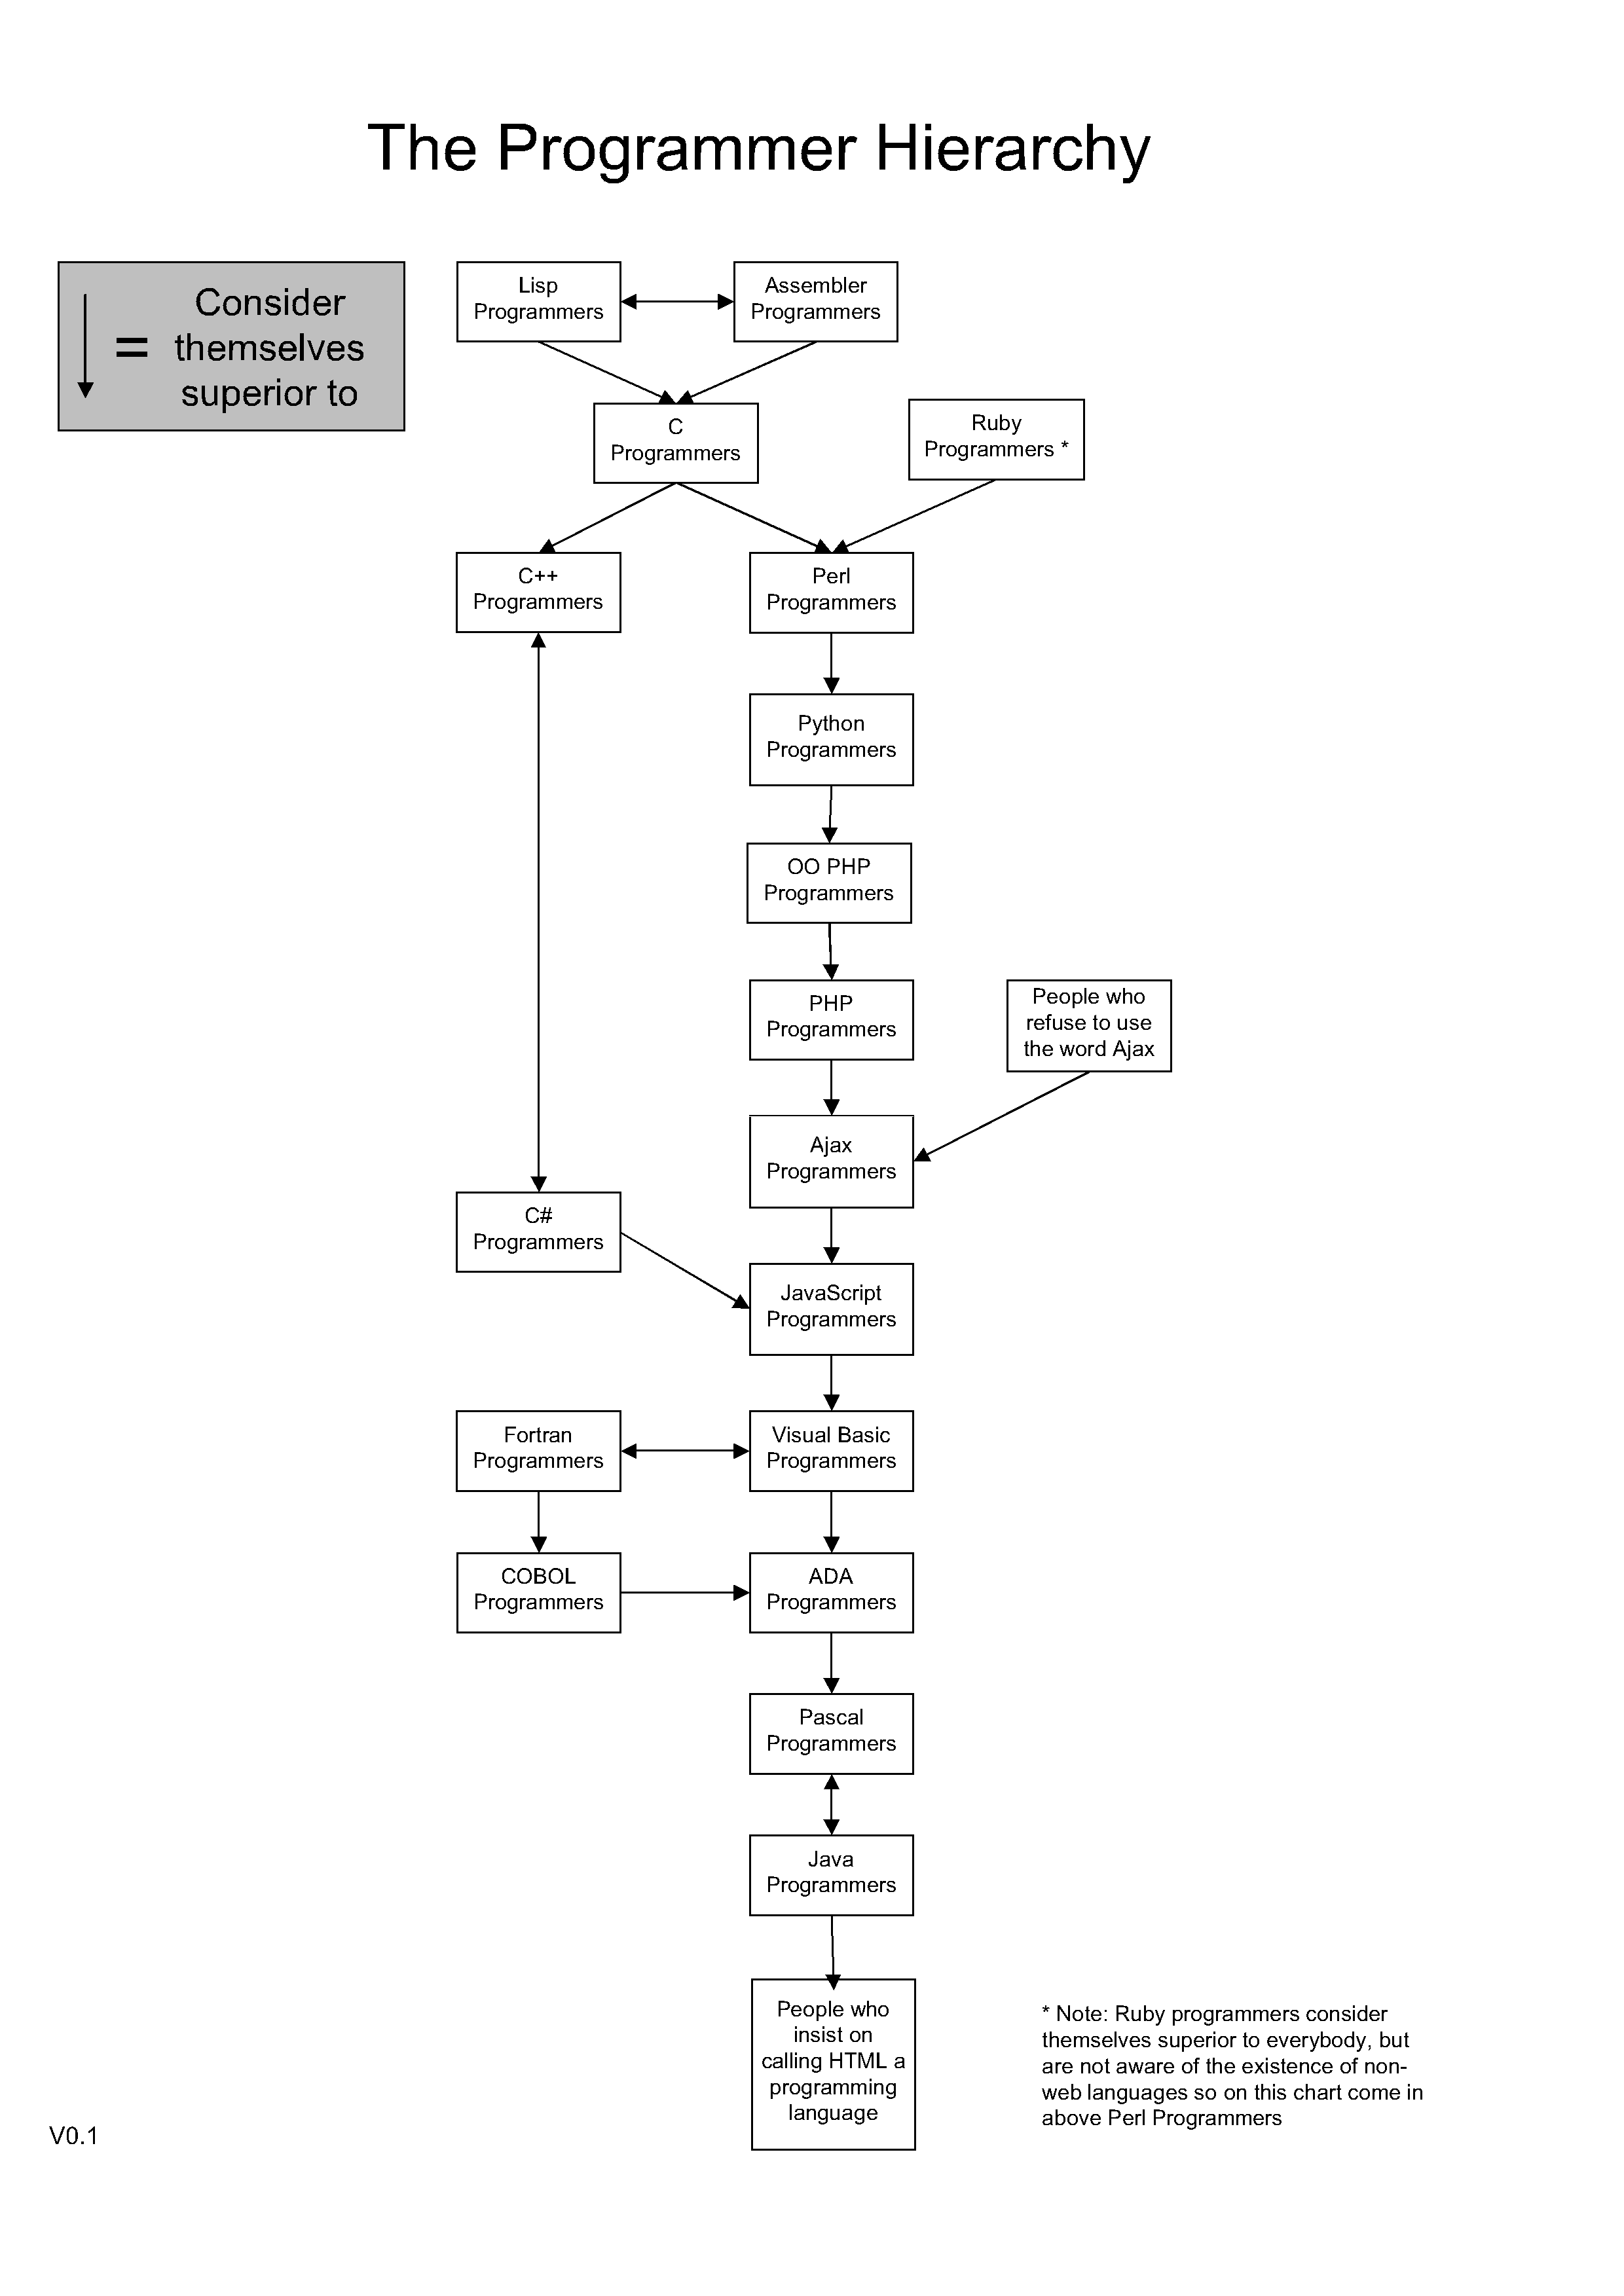
\includegraphics[scale=0.06]{guru}
	\end{figure}
\end{frame}

\section{Common Lisp}


\begin{frame}{Notacja polska kontra reszta świata}
	\begin{block}{Notacja infiksowa}
		\[2+2\]
		\[2+2\cdot 2\]
		\[(2+2)\cdot2\]
	\end{block}
	\pause
	\begin{block}{Notacja prefiksowa / polska / Łukasiewicza}
		\[+\ 2\ 2\]
		\[+\ 2\ \cdot \ 2\ 2\ =\ +\ \cdot\ 2\ 2\ 2\]
		\[\cdot\ 2\ +\ 2\ 2\ =\ \cdot\ +\ 2\ 2\ 2\]
	\end{block}
\end{frame}

\begin{frame}[fragile]
	\frametitle{Przykład}
	{\scriptsize \begin{lstlisting}
(defun invert-mod (x n)
  (multiple-value-bind (d r) (egcd x m)
    (when (= d 1) r)))
(defun chinskie-twierdzenie (lst)
  (let ((M (apply #'* (loop for i in lst collect (second i)))))
    (loop for i in lst sum (let* ((yi (second i))
                                  (Mi (floor M yi)))
                                 (* (third (multiple-value-list
                                                  (egcd yi Mi)))
                                    Mi
                                    (first i))))))
	\end{lstlisting}}
\end{frame}

\begin{frame}[fragile]
	\frametitle{Podstawowe wyrażenia 1}
	{\scriptsize \begin{lstlisting}
2
"Lustereczko, powiedz przecie"
(+ 2 2)
'(2 2)
(list 2 2)
\end{lstlisting}}
\end{frame}

\begin{frame}[fragile]
	\frametitle{Podstawowe wyrażenia 2}
	{\scriptsize \begin{lstlisting}
(let ((a 15)
      (b 16))
  (+ a b)
  5
  (+ a a 4 b))
(defparameter *glob1* 17)
(setf *glob1* 18) ; komentarz
\end{lstlisting}}
\end{frame}

\begin{frame}[fragile]
	\frametitle{Podstawowe wyrażenia warunkowe}
	{\scriptsize \begin{lstlisting}
(if warunek
  prawda
  falsz)
(when warunek
  prawda)

(if (and (= var 2) (print "Dwa!"))
  (progn
    (incf var)
    (- var 2))
  2)
(cond (warunek1 wynik1)
      (warunek2 wynik2)
  ; ...
      (warunekN wynikN))
\end{lstlisting}}
\end{frame}

\begin{frame}[fragile]
	\frametitle{Podstawowe pętle 1}
	{\scriptsize \begin{lstlisting}
(loop (print "Palenie procka"))
(let ((x 0))
  (loop (print "Petla")
        (if (>= x 10)
          (return)
          (incf x))))
\end{lstlisting}}
\end{frame}

\begin{frame}[fragile]
	\frametitle{Podstawowe pętle 2}
	{\scriptsize \begin{lstlisting}
(do (inicjacja_zmiennych)
  (warunek_konca zwracana_wartosc)
  instrukcje)

(do ((a 0 b)
     (b 1 (+ a b)))
  ((minusp (decf n) a)))

(dotimes (i 10)
  (print i))
(loop for i from 1 to 1000 by 3 when (oddp i) collect (* i i))
\end{lstlisting}}
\end{frame}

\begin{frame}[fragile]
	\frametitle{Tworzenie funkcji 1}
	{\scriptsize \begin{lstlisting}
(defun nazwa ([parametry]) tresc)

(defun kwadrat (x) (* x x))
(defun dodaj (a b) (+ a b))
(defun suma (&rest rest)
  (reduce #'+ rest))

#'suma --> #<FUNCTION SUMA>
\end{lstlisting}}
\end{frame}

\begin{frame}[fragile]
	\frametitle{Tworzenie funkcji 2}
	{\scriptsize \begin{lstlisting}
(defun double (x) (* x 2)

(setf (symbol-function 'double) #'(lambda (x) (* x 2)))

(mapcar #'(lambda (bla) (+ (kwadrat bla) 4)) '(1 2 3 4 5))

(defun make-adder (x)
  (lambda (a) (+ a x)))
(defparameter f (make-adder 7))
(funcall f 10)
\end{lstlisting}}
\end{frame}

\begin{frame}[fragile]
	\frametitle{Makra 1}
	{\scriptsize \begin{lstlisting}
(defmacro 3-way-if (ex A B C)
`(let ((__potencjalnyblad__ ,ex))
  (cond ((null __potencjalnyblad__ ,A)
        ((= __potencjalnyblad__ 0) ,B)
        (t ,C)))))
\end{lstlisting}}
\end{frame}


\begin{frame}{Podsumowanie}
	\begin{alertblock}{Najważniejsze}
		Język programowania jest narzędziem.
	\end{alertblock}
	\pause
	\begin{block}{A~może także\ldots}
		Warto poznawać alternatywy.
	\end{block}
\end{frame}

\begin{frame}{Literatura}
	\begin{itemize}
		\item{Peter Seibel - Practical Common Lisp}
		\item{Doug Hoyte - Let over Lambda}
		\item{Paul Graham}
			\begin{itemize}
				\item{ANSI Common Lisp}
				\item{On Lisp}
			\end{itemize}
		\item{Peter Norvig - Paradigms of Artificial Intelligence
			Programming, Case Studies in Common Lisp}
		\item{Conrad Barski - Land of Lisp}
		\item{(art.) Didier Verna - Beating C in Scientific Computing
			Applications}
		\item{(art.) B\o rge Svingen - When Lisp is faster than C}
		\item{(art.) Paul Graham - Beating the averages}
		\item{\texttt{http://student.agh.edu.pl/\textasciitilde gadek/lisp.pdf}}
	\end{itemize}
\end{frame}


\end{document}

